\chapter{Quantum Mechanics}\label{sec:qm}

Isaac Newton's famed remark, ``if I have seen further, it is by standing on the shoulders of giants'' could not be more true for the development of quantum mechanics \cite{Newton1675}. The 19th century gave birth to Maxwell's theory of electromagnetism which provided a theoretical framework for describing the transfer of energy through electromagnetic waves. At the same time, the likes of Boltzmann, Thomson, Joule and Clausius worked on combining heat with mechanical energy in the theory of thermodynamics. Together with classical mechanics these theories provided a very powerful framework for physics that led to numerous experiments being conducted to validate the theories to the highest precision possible. However, despite its successes there were still some unresolved issues. One of these issues was the origin and shape of the spectrum of a black body. Attempts by Rayleigh and Wien to explain the experimental data proved to be only sufficient in either the long or the short wavelength range. Max Planck had derived Wien's law in 1900 from entropic principles but as more data about the high frequency part of the spectrum became available he was forced to alter his arguments to account for the experimental data. By proposing that heated objects could only emit light in discrete chunks of energy $E_{\gamma} = h \nu$, where $h$ is Planck's constant and $\nu$ the frequency of the photon, he successfully derived a law that could explain the the spectrum for long and short wavelengths, now known as Planck's law,
\begin{equation*}
    u(\nu,T) = \frac{8 \pi h \nu^3}{c^3}\frac{1}{e^{h\nu / kT} - 1}.
\end{equation*}
Planck did not think that the quantization of energy implied that light had some discrete nature, he thought it a property of the radiation mechanism itself. It was not until 1905 that the discrete nature of light was proposed by Einstein who states in his paper \cite{Einstein1905}:  ``The energy [of a light ray] is not continuously distributed over an ever increasing volume, but it consists of a finite number of energy quanta, localized in space''. The idea of quantizing energy also led to a new model for the atom, introduced by Bohr in 1913. The previous model was Rutherford's planetary atom model, which could explain experiments about scattering quite well, but fell short when describing atomic line spectra. Between the publication of Bohr's model and the introduction of wave mechanics in the second decade, a lot of effort was put in developing a model of orbital shells that could explain the spectra of all elements up to Xenon. Quantum numbers were introduced to characterize the orbits, but there were still problems with the model. The Zeeman effect was still not well understood until in 1924 Pauli introduced the concept of spin. Around the same time, both Schr\"odinger and Heisenberg developed their own formalism to explain the atomic spectra. Heisenberg developed a strange method to calculate the atomic spectra and wrote a, in his own words, ``crazy'' paper about his findings. Born and his student Jordan recognized the procedures Heisenberg used as matrix operations, and so the theory got the name ``matrix mechanics". Parallel to this, Schr\"odinger wrestled with the idea that if particles behaved like waves, as proposed by De Broglie, then their must be some wave equation describing said waves. While Skiing in the Swiss Alps he found that equation that now carries his name,
\begin{equation*}
    i \hbar \frac{\partial \Psi(\mathbf{r},t)}{\partial t} = \left( \frac{\hbar^2}{2m} \nabla^2 - V(\mathbf{r}) \right) \Psi(\mathbf{r},t).
\end{equation*}
Paul Dirac showed the equivalence between the theories of Heisenberg and Schr- \"odinger in 1927, developing a more general mathematical framework that contained the work of both physicists. However there were still some kinks to work out, as stated by von Neumann: ``The method of Dirac, in no way satisfies the requirements of mathematical rigor'' \cite{Neumann1932}. Von Neumann's 1932 ``Mathematische Grundlagen der Quantenmechanik" would contain this mathematical rigor and to this day still forms the basis for a study into the mathematics of quantum mechanics. Parallel to the development of quantum mechanics, Einstein developed his theory of relativity. In thirty years the landscape of physics was transformed in a drastic manner, paving the way for what would be known as modern physics \cite{Cramer2016, terHaar1967}. 
\clearpage

\section{Postulates of Quantum Mechanics}

We will discuss the mathematical framework of quantum mechanics at lightning speed.
The postulates of quantum mechanics can be boiled down to the following statements:
\begin{enumerate}
    \item A physical state $\phi$ corresponds to a vector in a complex Hilbert space $\mathcal{H}$.
    \item The observable quantities of a quantum system are defined by self-adjoint operators $\Hat{A}$ on $\mathcal{H}$.
    \item The expectation value of an observable quantity $\Hat{A}$ for a system in a  state $\phi$ is given by the inner product $(\phi,\hat{A}\phi)$.
\end{enumerate}
A complex vector space $V$ is a set of elements $v\in V$ over a field $\mathbb{C}$, which is closed under addition and multiplication by scalars $\alpha\in \mathbb{C}$. This means that any linear combination of vectors $v = \sum_i \alpha_i v_i$, $v_i\in V$, $\alpha \in \mathbb{C}$ is also contained in $V$. A complex Hilbert space contains additional structure in the form of an inner product $(x,x)$ that produces a scalar in the complex plane. This inner product of $\mathcal{H}$ automatically defines a norm $\norm{x} \equiv \sqrt{( x, x )}$. To avoid unnecessary complication of the required mathematical background we will consider a finite Hilbert space $\mathbb{C}^n$ so that all operators are bounded by definition. This obviates the need to fully describe infinite dimensional metric spaces and the completeness of such spaces, which we do not need anyway. We also consider only systems with a non-degenerate eigenvalue spectrum.\newline 

\noindent An orthonormal set of vectors is always linearly independent and spans the full Hilbert space. It is common to write the vectors $x$ in the Dirac notation, where kets are denoted by $\ket{x}\in \mathcal{H}$ and bras by $\bra{x}\in \mathcal{H}^*$. The starred Hilbert space $\mathcal{H}^*$ refers to the dual space, and its elements are called covectors. The operation $\braket{x}{y}$ is not really an inner product, but a dual form. However, just like the inner product, it produces a scalar over the field of the respective vector space, which in the case is $\mathbb{C}^n$. If the Hilbert space is $n$-dimensional, then the standard basis $\mathbf{e}_i=\{\delta_{ij}\}^n$ is an orthonormal basis of the Hilbert space. We can write kets as vectors $\ket{\psi} = \sum_{i} a_i \mathbf{e}_i$ and bras as covectors $\bra{\psi} = \sum_{i} a_i^* \mathbf{e}_i^\dagger$ with the additional operation of the standard dot-product. This definition ensures that the norm $\sqrt{\braket{\psi}{\psi}}$ produces a real number larger than zero. We can convert a bra into ket by taking the conjugate transpose operation$\bra{\psi}^\dagger\rightarrow\ket{\psi}$.\newline

\noindent In order to perform measurements or transform a physical system, we require operators that act on these vectors (also known as state vectors). Operators in quantum physics are described in the language of abstract linear operators that act as basis transformations between two vector spaces. These operators are most often denoted by a hat: $\hat{A}$. In general two operators do not commute $\comm{\Hat{A}}{\Hat{B}} = \hat{A}\hat{B}-\hat{B}\hat{A}\neq 0$. Similar to bras and kets, there is a dual operator that works on elements of the dual vector space. These operators act on the states as $\braket{\psi}{(\Hat{A}\psi)} = \bra{\psi}\Hat{A}\ket{\psi}$ and $\braket{(\Hat{A} \psi)}{\psi)} = \bra{\psi}\Hat{A}^\dagger\ket{\psi}$. In other words, $\hat{A}$ works on kets, while $\hat{A}^\dagger$ works on bras. It can be shown that operators can be represented by matrices and their operations of matrix addition and matrix multiplication, e.g. they are isomorphic to the abstract language of linear operators $\hat{A} \equiv \mathbf{A}$.
Writing these matrices in terms of the standard basis gives ${A}^\dagger_{ij} = \mathbf{e}_i^T{A}^\dagger \mathbf{e}_j = (\mathbf{e}_j^T {A} \mathbf{e}_i)^* = {A}^*_{ji}$ by conjugate symmetry of the inner product, so $\mathbf{A}^\dagger$ is the conjugate transpose of $\mathbf{A}$.\newline

\noindent Define a projector operator as $P_i = \ket{v_i}\bra{v_i}$, this operator projects the component of some arbitrary state $\ket{\phi}$ out with respect to the basis $\{\ket{v_i}\}$,
\begin{equation*}
    P_i \ket{\phi} = \ket{v_i}\bra{v_i} \sum_j a_j\ket{v_j} = \ket{v_i} \delta_{ij} a_j = a_i \ket{v_i}.
\end{equation*}
Furthermore, the sum of projectors equals the identity operation,
\begin{equation*}
    \left(\sum_i \ket{v_i}\bra{v_i}\right)\ket{\phi} = \sum_{i,j} \ket{v_i}\bra{v_i} a_j \ket{v_j} = \sum_{i,j} a_j \ket{v_i} \delta_{ij} = \ket{\phi} .
\end{equation*}
An operator is self-adjoint if $\Hat{A} = \Hat{A}^\dagger$. This is also referred to as a Hermitian operator. For every physical property $\mathcal{A}$ there exists an observable $\hat{A}$ that is a Hermitian operator on $\mathcal{H}$. The eigenvalues of this operator correspond to the possible values of the underlying physical property. If an operator $\hat{A}$ is Hermitian, there exists an orthonormal basis $\{\ket{u_i}\}$ of eigenvectors of $\hat{A}$, so that the matrix representation of $\hat{A}$ is diagonal with eigenvalues filling the diagonal of the matrix (assuming a non-degenerate spectrum). From the definition of the Hermitian operator we see that these eigenvalues must be real,
\begin{equation}
    \hat{A} = \sum_i \lambda_i \ket{u_i}\bra{u_i} \label{eq:observable}.
\end{equation}
This theorem is called the Spectral Theorem and is quite convenient because it allows to work with diagonal matrices, simplifying computations considerably. It also provides a way to relate the mathematical framework of quantum mechanics to the real world by measuring the eigenvalues of the operator we are interested in. Most often this operator is the Hamiltonian $\hat{H}\equiv H$ of the system, which contains the sum of potential and kinetic energies. The Schr\"odinger equation then tells us how the physical states of the system evolve,
\begin{equation*}
    i \hbar \frac{\partial \ket{\psi}}{\partial t} = H  \ket{\psi}.
\end{equation*}
Obtaining information about some observable of a quantum system can be done through measurement. However, to obtain information about this system we must somehow interfere with the system. The Born rule bridges the quantum world with the classical world. Let $p_i = |\braket{u_i}{\psi}|^2$ be the probability that we measure the eigenvalue $\lambda_i$ for some self-adjoint operator $\hat{A}$, where $\ket{u_i}$ is the corresponding eigenvector of $\hat{A}$. The complex numbers $a_i$ in $\ket{\psi}=\sum_i a_i \ket{v_i}$ are called probability amplitudes. After the measurement, the system collapses to the state $\ket{u_i}$ and measuring it again will return the eigenvalue $\lambda_i$ with probability $1$, this is known as wave function collapse. We can understand this behaviour by considering measurements to be projection operators consisting of eigenstates of observables,
\begin{equation*}
    p_i = \braket{\psi}{u_i}\braket{u_i}{\psi} = \bra{\psi} P_i \ket{\psi}.
\end{equation*}
Since the result of single measurement is probabilistic, we are usually more interested in the average behaviour of an observable,
\begin{equation*}
    \langle \hat{A}\rangle = \bra{\psi} \hat{A} \ket{\psi}.
\end{equation*}
The interpretation of quantum mechanics as a phenomenological theory is known as the ``Copenhagen Interpretation". According to this interpretation, there is a discontinuity between the quantum regime and the classical regime, bridged by invoking an observer that collapses the wave function of the system. This explanation is unsatisfactory to many physicists and as such, there exist many proposals to solve this so called ``measurement problem" \cite{Schlosshauer2005}. The philosophical debate on this topic spans almost a century and we will refrain from adding anything to it, for a detailed overview the reader is referred to \cite{Myrvold2018}.

\section{Tensor Products}\label{sec:tens_prod}

In classical physics we can describe the total phase space of a composite system as the Cartesian product of the subsystem phase spaces. For example Consider two systems $H(x)$ and $G(y)$, then the possible states for the composite system $K = H \times G = \{(x,y) | x\in H \text{ and } y\in G\}$ with $\dim K = \dim H + \dim G$. To describe composite quantum systems we require more mathematical tools, in the form of the tensor product. The formal definition is a bit abstract, but for completeness we will include it here. The tensor product of two vector spaces $V$ and $W$ is the map $\otimes: V\times W\rightarrow V\otimes W$ so that for $v\in V$, $w\in W$ and $\hat{v}\in V^*$, $\hat{w}\in W^*$ we have $(v\otimes w)(\hat{v},\hat{w}) = \hat{v}(v) \otimes \hat{w}(w)$. For linear operators $\hat{A}:V\rightarrow V^\prime$, $\hat{B}:W\rightarrow W^\prime$ we have that $(\hat{A}\otimes\hat{B})(v\otimes w) = (\hat{A}v)\otimes (\hat{B}w)$. \newline

\noindent This product establishes a connection between two vector spaces, its basis vectors and the operators that can be constructed in this new space. Let $\mathcal{H}_A$ and $\mathcal{H}_B$ be two Hilbert spaces. The tensor product space $\mathcal{H} = \mathcal{H}_A\otimes \mathcal{H}_B$ is a vectorspace of dimension $\dim(\mathcal{H}) = \dim(\mathcal{H}_A)\cdot \dim(\mathcal{H}_B)$, with elements of $\mathcal{H}$ being linear combinations of $\ket{\psi_A}\otimes\ket{\psi_B}$, where $\ket{\psi_A}\in\mathcal{H_A}$ and $\ket{\psi_B} \in \mathcal{H_B}$. 
If $\{\ket{v_i}\}$ and $\{\ket{v_j}\}$ are orthonormal bases for $\mathcal{H}_A$ and $\mathcal{H}_B$, then $\{\ket{v_i} \otimes \ket{v_j}\}$ is a basis of $\mathcal{H}$. In the language of matrix representations we use the Kronecker product to calculate the tensor product of vectors and matrices,
\begin{equation*}
    \ket{\psi} = \ket{\psi_A}\otimes\ket{\psi_B} = 
    \begin{pmatrix}
        a_1 \\
        \vdots\\
        a_n
    \end{pmatrix}
    \otimes
    \begin{pmatrix}
        b_1 \\
        \vdots\\
        b_m
    \end{pmatrix}
    =
    \begin{pmatrix}
    a_1 \begin{pmatrix}
        b_1 \\
        \vdots\\
        b_m
    \end{pmatrix}\\
    \vdots\\
    a_n \begin{pmatrix}
        b_1 \\
        \vdots\\
        b_m
    \end{pmatrix}
    \end{pmatrix},
\end{equation*}
where $\ket{\psi}$ is indexed by $a_i b_j$. For operators this is extended to
\begin{align*}
    \hat{U} = 
    \hat{A}\otimes\hat{B} & \equiv \mathbf{A}\otimes\mathbf{B} = 
    \begin{pmatrix}
        a_{11} & \ldots & a_{1n} \\
        \vdots & \ddots & \vdots\\
        a_{n1} & \ldots & a_{nn}
    \end{pmatrix}
    \otimes
    \begin{pmatrix}
        b_{11} & \ldots & b_{1m} \\
        \vdots & \ddots & \vdots\\
        b_{m1} & \ldots & b_{mm}
    \end{pmatrix}\\
    &=
    \begin{pmatrix}
        a_{11} \begin{pmatrix}
        b_{11} & \ldots & b_{1m} \\
        \vdots & \ddots & \vdots\\
        b_{m1} & \ldots & b_{mm}
    \end{pmatrix} & \ldots & a_{1n} \begin{pmatrix}
        b_{11} & \ldots & b_{1m} \\
        \vdots & \ddots & \vdots\\
        b_{m1} & \ldots & b_{mm}
    \end{pmatrix}\\
        \vdots & \ddots & \vdots\\
        a_{n1} \begin{pmatrix}
        b_{11} & \ldots & b_{1m} \\
        \vdots & \ddots & \vdots\\
        b_{m1} & \ldots & b_{mm}
    \end{pmatrix}& \ldots & a_{nn}\begin{pmatrix}
        b_{11} & \ldots & b_{1m} \\
        \vdots & \ddots & \vdots\\
        b_{m1} & \ldots & b_{mm}
    \end{pmatrix}
    \end{pmatrix},
\end{align*}
so $\hat{U}$ is indexed by $A_{ij}B_{kl}$.

\section{Density Matrix}\label{sec:density_matrix}

Up to this point we have only considered state vectors as a description of a system, with probability amplitudes assigned to each possible state. In an experimental setting we have to repeat a certain measurement a number of times to obtain statistics of some observable. This assumes that we can prepare the system identically for each measurement, but this might prove to be difficult in practice. To deal with this problem we define a density matrix $\rho$ to describes a statistical ensemble of quantum systems.
A density matrix $\rho$ for an $n$-dimensional quantum system $\mathcal{H}$ is a self-adjoint matrix with the properties
\begin{enumerate}
    \item $\Tr{\rho}=1$
    \item $\rho$ is non-negative, e.g. has only eigenvalues $\geq 0$
    \item $\langle \hat{A} \rangle = \Tr{\rho \hat{A}}$
    \item $\rho = \sum_i \lambda_i \ket{v_i}\bra{v_i}$ where $\{\ket{v_i}\}$ is an orthogonal basis
\end{enumerate}
In terms of statevectors we have for two systems A and B that the combined state can always be written in the form
\begin{equation}
    \ket{\psi} = \sum_i c_{ij} \ket{\psi^A_i} \otimes \ket{\psi^B_j}
    \label{eq:pure_state}.
\end{equation}
We say that the system is in a pure state if the density matrix is given by a single state vector,
\begin{equation}
    \rho^{pure} = \ket{\psi} \bra{\psi} \label{eq:rho_pure}.
\end{equation}
The system is in a mixed state if it can be written in terms of a linear combination of pure states,
\begin{equation}
    \rho^{mixed} = \sum_i p_i \ket{\psi}_i \bra{\psi}_i \label{eq:rho_mixed}.
\end{equation}
with $\sum_i p_i =1$ to ensure that the trace is 1. In other words, $p_i$ is the probability $0\leq p_i \leq 1$ of obtaining a certain pure state when preparing the system. If $n=1$ and $p = 1$ then the system is in a pure state. If the state is pure then the matrix $\rho$ is idempotent, $\rho^2=\ket{\psi}\bra{\psi}\ket{\psi}\bra{\psi}=\rho$ and rank one. The average behaviour of a mixed system is calculated with the trace,
\begin{equation}
    \expval{\hat{A}} = \Tr{\hat{A}\rho} \label{def:density_mat}.
\end{equation}

\section{Qubits}\label{sec:qubits}

The study of quantum information concerns itself with understanding how information is contained and propagated in quantum systems. An essential ingredient for this study is the qubit: A two level quantum system and quantum equivalent of the classical bit. The easiest examples of a qubit in the physical world is the a spin-$\frac{1}{2}$ particle or the vertical and horizontal polarization of a photon.  When working with spin-$\frac{1}{2}$ states the canonical choice of basis are the eigenstates of the Pauli $\sigma^z$ operator,
\begin{equation*}
    \sigma_z = \begin{pmatrix}
                    1 & 0\\
                    0 & -1  
            \end{pmatrix} \quad \text{with} \quad
            \ket{0} = \mathbf{e}_0 = \begin{pmatrix}
                    1 \\
                    0  
            \end{pmatrix}
            \quad 
            \ket{1} = \mathbf{e}_1 =
            \begin{pmatrix}
                    0 \\
                    1  
            \end{pmatrix}.
\end{equation*}
The two basis define the computational basis $\{\ket{i}\}$, which is commonly used in quantum computing. 
We can write the total state of a qubit as $\ket{\psi} = a \ket{0} + b \ket{1}$ with $|a|^2 + |b|^2 = 1$. Because the only constraint on the state is the normalization of the probability amplitudes $a,b \in \mathbb{C}$ we can rewrite this more generally as
\begin{equation*}
    \ket{\psi} = e^{i\gamma}\left(\cos \frac{\theta}{2}\ket{0} +  e^{i\phi}\sin\frac{\theta}{2}\ket{1} \right),
\end{equation*}
with $\theta$, $\phi$, $\gamma \in \mathbb{R}$. Due to the complex conjugation in the Born rule the term $e^{i\gamma}$ has no observable effects it can be left out, so the qubit is fully defined by the two angles $\theta$ and $\phi$ \cite{Nielsen2011},
\begin{equation}
    \ket{\psi} = \cos \frac{\theta}{2}\ket{0} +  e^{i\phi}\sin\frac{\theta}{2}\ket{1}
    \label{eq:bloch}.
\end{equation}
The angles $\theta$ and $\phi$ describe a point on a sphere with radius 1 called the Bloch sphere which can be seen in figure \ref{fig:bloch_sphere}. 
\begin{figure}[ht!]
    \centering
    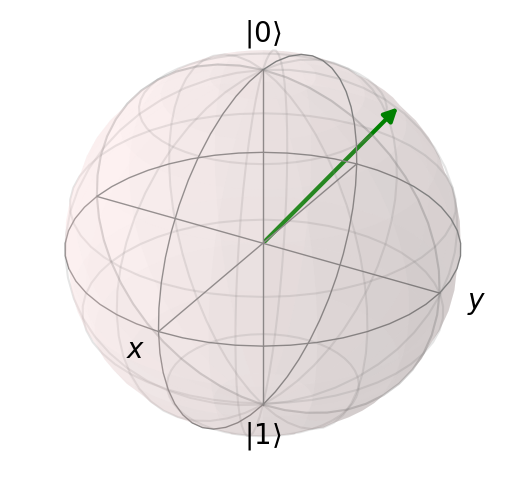
\includegraphics[width=0.7\textwidth]{figures/chapter1/bloch_sphere.png}
    \caption{The Bloch sphere of a qubit state with $\theta = \frac{1}{4}\pi$ and  $\phi = \frac{3}{4}\pi$. The vector is in spherical coordinates written as $\mathbf{a} = (\sin(\theta) \cos(\phi), \sin(\theta) \sin(\phi), \cos(\theta))$  \cite{Johansson2013}.}
    \label{fig:bloch_sphere}
\end{figure}
For mixed states we can also use the Bloch sphere. We know that a density matrix $\rho$ is a trace 1, Hermitian matrix. This means that it can be written in terms of the Pauli basis,
\begin{align}
    \rho &= \frac{1}{2} (\mathbb{1} + \sum_{k} r^k \sigma^k ) = \frac{1}{2}(\mathbb{1} + \mathbf{r} \cdot \bm{\sigma}) =  
            \begin{pmatrix}
                1 + r^z & r^x - i r^y\\
                r^x + i r^y & 1 - r^z  
            \end{pmatrix}\nonumber,\\
    \sigma_x &= \begin{pmatrix}
                    0 & 1\\
                    1 & 0  
            \end{pmatrix} \quad,
    \sigma_y = \begin{pmatrix}
                    0 & -i\\
                    i & 0  
            \end{pmatrix} \quad,
    \sigma_z = \begin{pmatrix}
                    1 & 0\\
                    0 & -1  
            \end{pmatrix} \label{eq:pauli_mats}.
\end{align}
The vector $\mathbf{r}$ is called the Bloch vector with $\norm{\mathbf{r}} \leq 1$ and equality when the state $\ket{\psi}$ is pure. The Bloch sphere visualization can be useful to provide some insight into how individual qubits are affected by operators. We will use this in chapter 3 to show how the quantum a classical distribution over a qubit differs from the quantum equivalent.\newline

\noindent When working with a multi-qubit system we often use the shorthand notation $\ket{00}\equiv \ket{0} \otimes \ket{0}$, for instance a state $\ket{00}\bra{11} = (\ket{0}\otimes \ket{0}) (\bra{1}\otimes \bra{1}) = \ket{0}\bra{1} \otimes \ket{0}\bra{1}$ by the previous definition of the tensorproduct. Visualizing the density matrix becomes harder since the length of the vector scales with $(n^2 - 1)$ for a $n\times n$ density matrix. For 2 qubits this would already give a 15 dimensional vector that we would have to visualize.

\section{Partial Traces}\label{sec:partial_tr}

Just like in classical mechanics, we might be interested in only a smaller section of the entire phase space, for instance a single particle. We can trace out degrees of freedom in quantum physics by taking the partial trace of the density matrix. This will outline some of the strange properties of quantum physics, where looking at subsystems decreases the knowledge of the entire system, as opposed to increasing it. \newline

\noindent Let $\rho_{AB}$ be the density matrix in a complex Hilbert space $\mathcal{H}_A\otimes\mathcal{H}_B$. We can find the reduced density matrix $\rho_A\in \mathcal{H}_A$  by taking the partial trace over the subsystem $B$,
\begin{align}
    \rho_A \equiv \Tr_B(\rho_{AB}).
\end{align}
The partial trace is the linear map $\Tr_B\: : \:\mathcal{L}(\mathcal{H}_A\otimes\mathcal{H}_B) \rightarrow \mathcal{L}(\mathcal{H}_A)$ where $\mathcal{L}(V)$ is the space of linear operators on the vector space $V$. This operation is then given by
\begin{align}
    \Tr_B(\rho_{AB}) \equiv \rho_A \Tr_B(\rho_B).
\end{align}
This approach looks straightforward enough, we remove the degrees of freedom belonging to the subsystem we are not interested in. Consider the system in the product state $\rho_{AB} = \rho_A \otimes \rho_B$ with $\rho_A\in \mathcal{H}_A$, $\rho_B\in \mathcal{H}_B$ and $\rho_{AB}\in \mathcal{H}_A\otimes\mathcal{H}_B$. Performing the partial trace over $B$ gives gives $\rho_A \Tr_B(\rho_B) = \rho_A$, and vice versa for $A$.\newline
We can also imagine a system $\rho_{AB} = \sum_i p^i \rho^i_A\otimes\rho^i_B$ consisting of two qubits. For instance the famous Bell State,
\begin{align}
    \ket{\psi} = \frac{1}{\sqrt{2}}(\ket{00}+\ket{11})
    \label{eq:bell_state},
\end{align}
has a corresponding density matrix
\begin{align}
    \rho = \ket{\psi}\bra{\psi} = \frac{1}{2}(\ket{00}\bra{00} + \ket{11}\bra{00} + \ket{00}\bra{11} + \ket{11}\bra{11}).
\end{align}
Remember that a state $\ket{00}\bra{11} \equiv \ket{0}_A\bra{1}_A \otimes \ket{0}_B\bra{1}_B$. If we trace out qubit $B$, we get 
\begin{align*}
    \Tr_B(\rho) = & \frac{1}{2}(\Tr_B(\ket{0}_A\bra{0}_A \otimes \ket{0}_B\bra{0}_B) + \Tr_B(\ket{1}_A\bra{0}_A \otimes \ket{1}_B\bra{0}_B) +\\
    & \Tr_B(\ket{0}_A\bra{1}_A \otimes \ket{0}_B\bra{1}_B) +\Tr_B( \ket{1}_A\bra{1}_A \otimes \ket{1}_B\bra{1}_B))\\
     = & \frac{1}{2}(\ket{0}_A\bra{0}_A + \ket{1}_A\bra{1}_A).
\end{align*}
Notice that this state is a mixed state, a linear combination of density matrices. For the composite system $\rho$ we have a pure state, which indicates full knowledge of the system. But, for the subsystem A we are uncertain of the state that it is in, since we have probability $\frac{1}{2}$ of finding the system in either state $\ket{0}$ or $\ket{1}$. Looking at a subsystem decreases the knowledge of the entire system \cite{Nielsen2011,Vershynina2013}!

\section{Entanglement}\label{sec:entanglement}

In the previous paragraph we have introduced the notion of entanglement: The properties of a system cannot be described solely in terms of the individual subsystems. Measuring subsystem A impacts the information we can obtain about subsystem B. Despite its success, this "spooky action at a distance" was a fundamental problem for quantum physics according to Einstein, Podolsky and Rosen \cite{EPR}. It would take 30 years before Bell would prove that a local theory could not be consistent with quantum theory. The concept of entanglement has received a lot of renewed interest in the 1990s and 2000s with the rise of quantum computing and quantum information. A full theory of entanglement is still not realized, mostly because of its complex structure. \newline
The origin of entanglement is the tensor product of subsystem Hilbert spaces. For some composite system $\mathcal{H} = \bigotimes_i^n \mathcal{H}_i$ we have an orthonormal basis $\{\ket{v_i} = \ket{v_{i_1}} \otimes \ket{v_{i_2}} \otimes \ldots \otimes \ket{v_{i_n}}\}$ with indices $i_j=1,\ldots ,\text{dim}(H_i)$ . The total state of the system is described by
\begin{equation*}
    \ket{\psi} = \sum_i a_i \ket{v_i}.
\end{equation*}
with $\sum_i a_i^2 = 1$, $a_i \in \mathbb{C}$ and this can in general not be described as a product of states of individual subsystems,
\begin{equation*}
    \ket{\psi} \neq \ket{\psi_1}\otimes \ket{\psi_2} \otimes \ldots \otimes \ket{\psi_n}.
\end{equation*}
This inequality expresses formally the phenomenon of entanglement. If the total system consists of two subsystems, the system is called bipartite. If it consists of $n$ subsystems it is called multipartite. The above definition is only valid for a pure system $\rho = \ket{\psi}\bra{\psi}$. In the case of a mixed state, we have to extend the definition with density matrices. A mixed state of $n$ systems is entangled if it cannot be written as a linear combination of product states,
\begin{equation}
    \rho \neq \sum_i p_i \rho_1^i \otimes \ldots \otimes \rho^i_n
    \label{eq:entangled}.
\end{equation}
If such a combination does exist, then the states are called separable. In practice it is hard to decide if states are separable or entangled based on this definition, we therefore look to other ways of measuring entanglement. The study of the quantification of entanglement is a vast field of research, and the proposals for entanglement measures are numerous \cite{Horodecki2009}.\newline
A key concept in classical information theory is the so called Shannon entropy which says something about the average information we gain when we learn the value of a random variable $X$. We can also view this as a measure of uncertainty about $X$ before we learn its value \cite{Nielsen2011},
\begin{equation}
    H_s(X) \equiv H_s(p_1,...,p_n)\equiv -\sum_i p_i \log_2 p_i\label{eq:shannon}.
\end{equation}
This definition is motivated by Shannon to represent the minimal amount of bits required to reconstruct the information produced by some source. There is a quantum equivalent of this called the von Neumann entropy which extends this definition to density matrices,
\begin{equation*}
   S(\rho) \equiv -\Tr{\rho \log_2{\rho}}= - \sum_i \lambda_i \log_2 \lambda_i,
\end{equation*}
by diagonalization of $\rho$ where $\lambda_i$ are the eigenvalues of $\rho$. This definition reduces to the classical definition in the case that $\rho$ is diagonal. Note that both the Shannon and von Neumann entropy lie between $0$ and $1$ and we assume that $0 \log_2 0 = 0$. \newline
For a bipartite system we can quantify the amount of entanglement with the relative entanglement entropy, which is defined as the von Neumann entropy of the reduced density matrix,
\begin{equation*}
    S(\rho_A) = -\Tr{\rho_A \log_2{\rho_A}}\label{eq:vn_entropy_entanglement}.
\end{equation*}
Consider a system of two qubit A and B of the form,
\begin{equation*}
    \ket{\psi} = \frac{1}{\sqrt{2a^2-2a +1}} \left(a \ket{00} + (1 - a)\ket{11} \right).
\end{equation*}
We can trace out qubit B to obtain the reduced density matrix $\rho_A$ and calculate the entropy as a function of $a$, this can be seen in figure \ref{fig:bell_state_a}.
\begin{figure}[ht!]
    \centering
    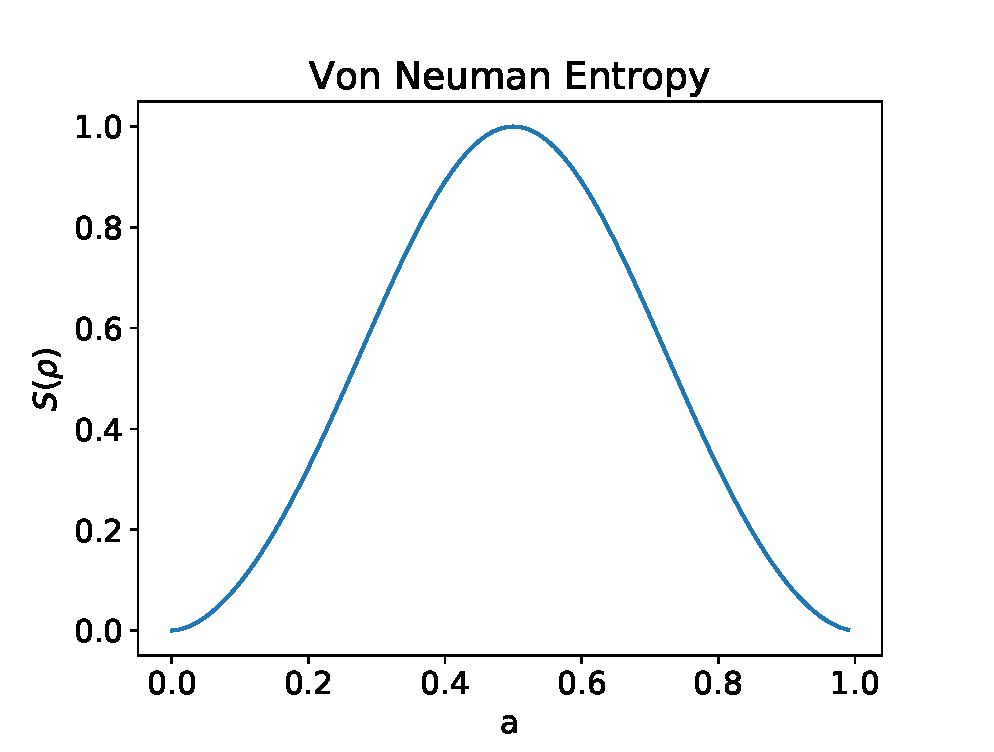
\includegraphics[width=0.7\textwidth]{figures/chapter1/bell_state_a.eps}
    \caption{The von Neumann entropy for a parameterized state. For $a=0.5$ the relative entropy is maximal and corresponds to the Bell state in equation \ref{eq:bell_state}.}
    \label{fig:bell_state_a}
\end{figure}
This definition of a quantum entropy works only for pure states. If we consider a simple mixed state of non-entangled systems we can see that the von Neumann entropy becomes maximal, where we would like it to be zero. For instance, consider the following systems and corresponding mixed state ensemble,
\begin{align*}
    \rho^A_1 &= \ket{0} \bra{0} \text{, } \rho^B_1 = \ket{1} \bra{1} \text{, } \rho^A_2 = \ket{1} \bra{1} \text{, }
    \rho^B_2 = \ket{0} \bra{0}\\
    &\text{choose $p_1=p_2=\frac{1}{2}$}\\
    \rho &= \sum_i p_i (\rho^A_i \otimes \rho^B_i) = \frac{1}{2} \left( \overbrace{\rho^A_1 \otimes \rho^B_1}^{\text{pure state}} + \overbrace{\rho^A_2 \otimes \rho^B_2}^{\text{pure state}}\right).
\end{align*}
If we now try to calculate the entropy for this mixed system, we will find that the subsystem entropy is maximal, while according to the definition of equation \ref{eq:entangled} this system is not entangled since it is a linear combination of density matrix product states,
\begin{align*}
    \Tr_A{\rho} = \frac{1}{2} \left( \rho^B_1 + \rho^B_2 \right)\\
    S(\rho_B) = -2 (\frac{1}{2} \log_2{\frac{1}{2}}) = 1.
\end{align*}
So a bipartite mixed state has maximum entropy while being not entangled. This indicates that finding a good measure of entanglement might not be as simple as it seems. The literature on this subject is extensive \cite{Horodecki2009}.